\cleardoublepage
\chapter{DOKUMENTASI KEGIATAN KERJA PRAKTIK}
\setcounter{figure}{0}
\renewcommand{\thefigure}{\thechapter.\arabic{figure}}

\begin{figure}[H]
    \centering
    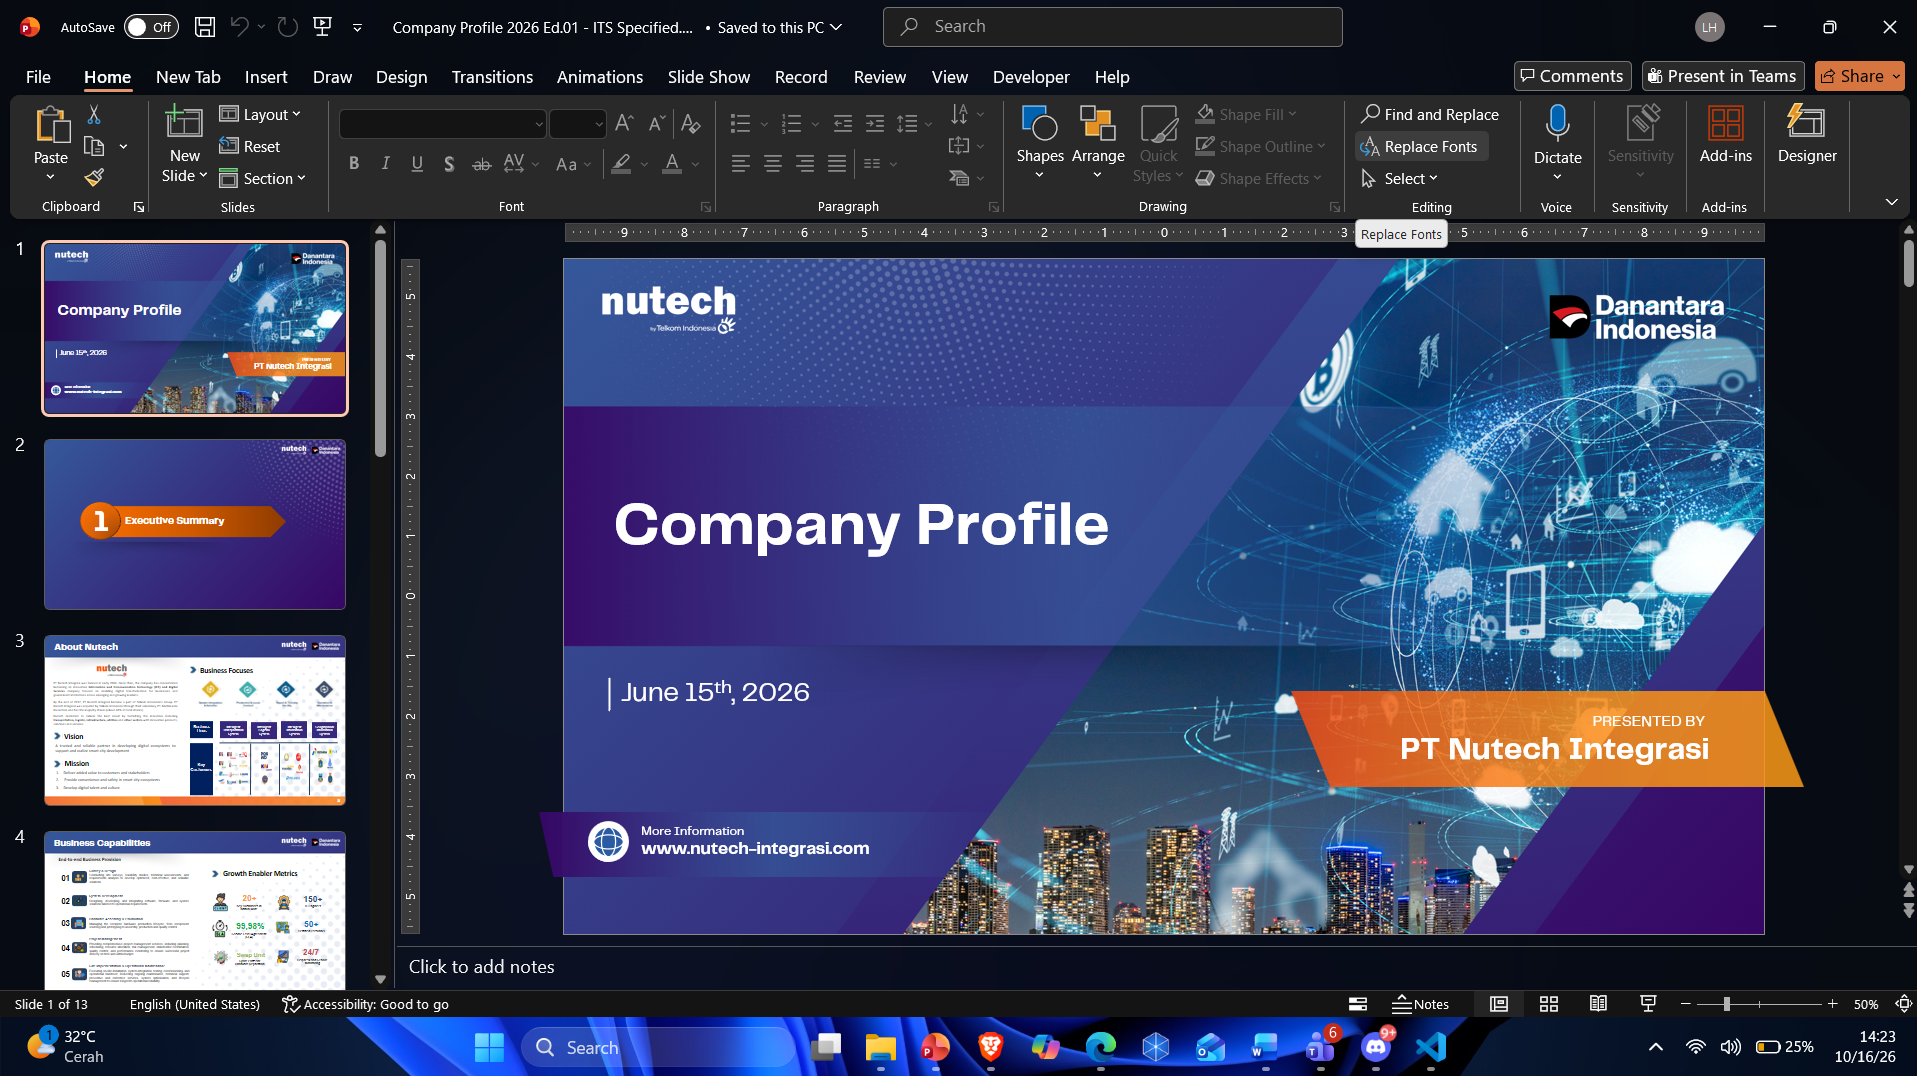
\includegraphics[width=0.85\textwidth]{images/Companny.png}
    \caption{Profil perusahaan PT Nutech Integrasi}
\end{figure}

\begin{figure}[H]
    \centering
    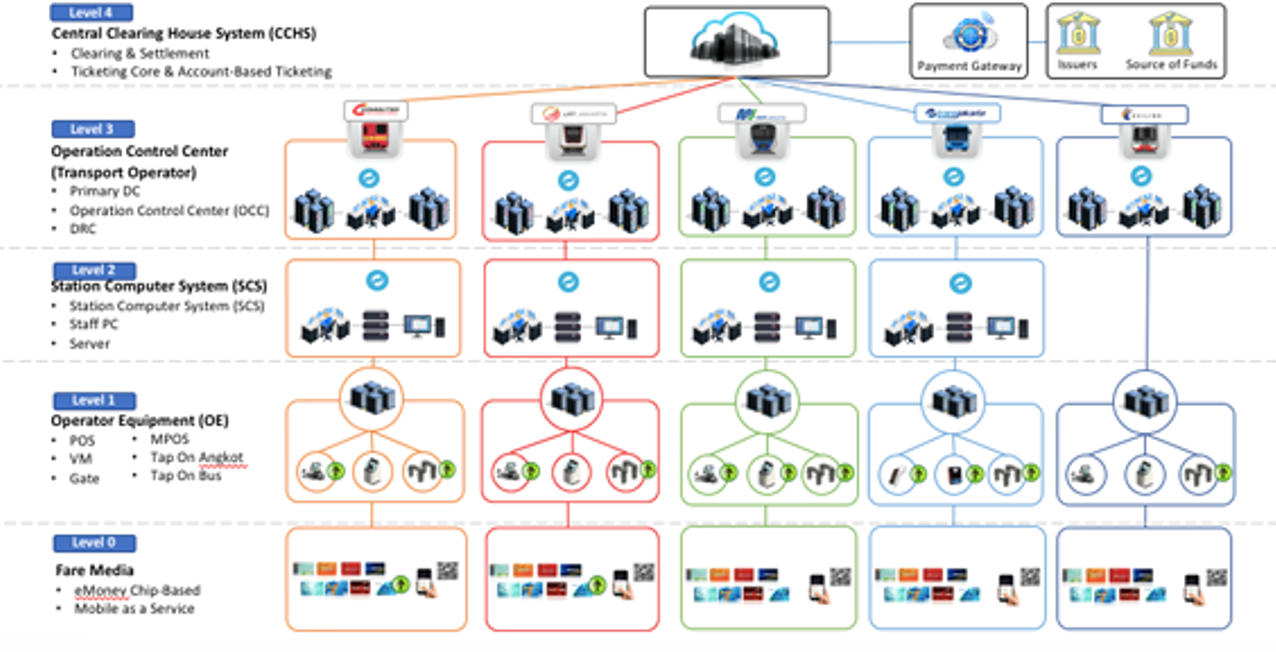
\includegraphics[width=0.95\textwidth]{images/Diagram Arsitektur Sistem AFC.png}
    \caption{Diagram arsitektur sistem \textit{Automatic Fare Collection} (AFC)}
\end{figure}

\begin{figure}[H]
    \centering
    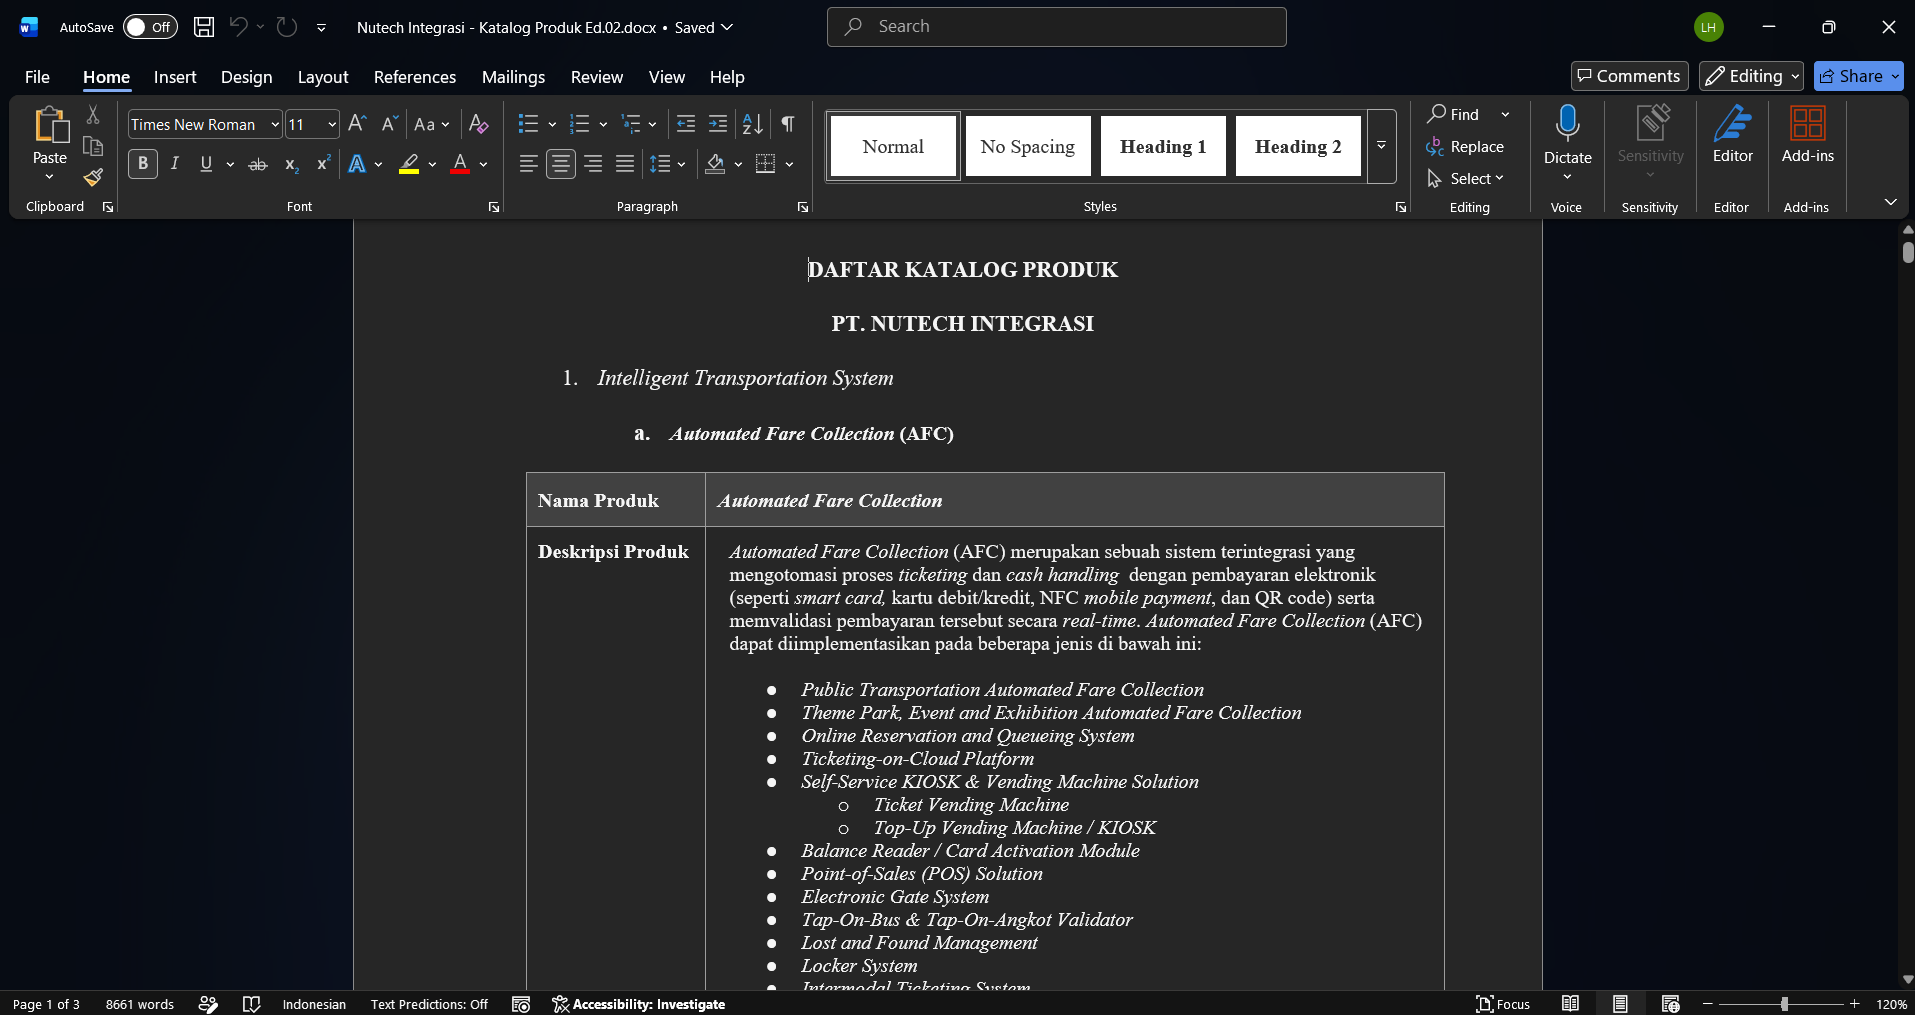
\includegraphics[width=0.85\textwidth]{images/Katalog.png}
    \caption{Dokumen katalog produk PT Nutech Integrasi}
\end{figure}

\begin{figure}[H]
    \centering
    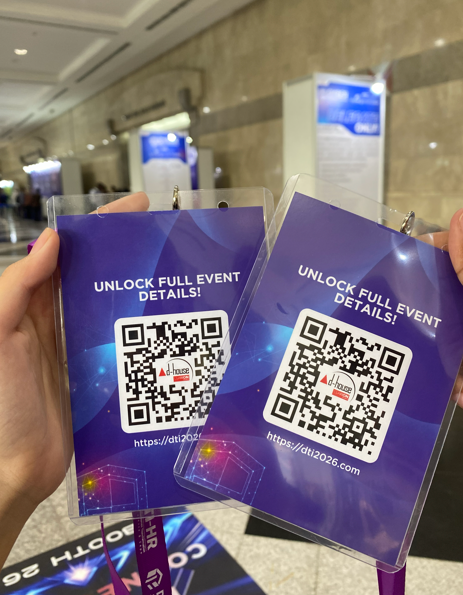
\includegraphics[width=0.85\textwidth]{images/kegiatan1.png}
    \caption{Dokumentasi kegiatan kerja praktik 1}
\end{figure}

\begin{figure}[H]
    \centering
    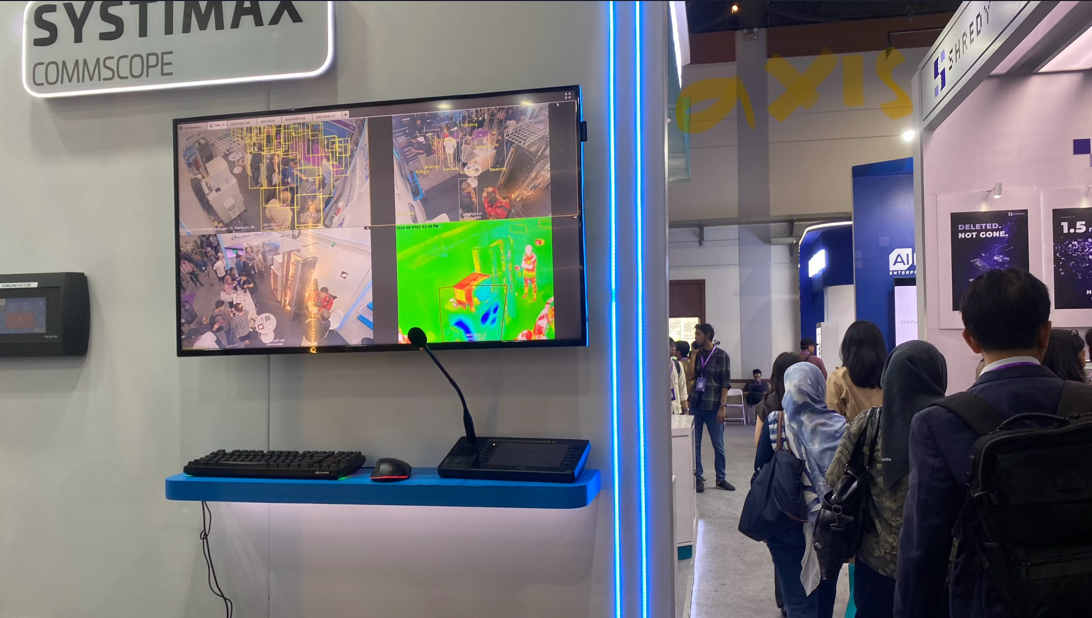
\includegraphics[width=0.85\textwidth]{images/kegiatan2.png}
    \caption{Dokumentasi kegiatan kerja praktik 2}
\end{figure}

\begin{figure}[H]
    \centering
    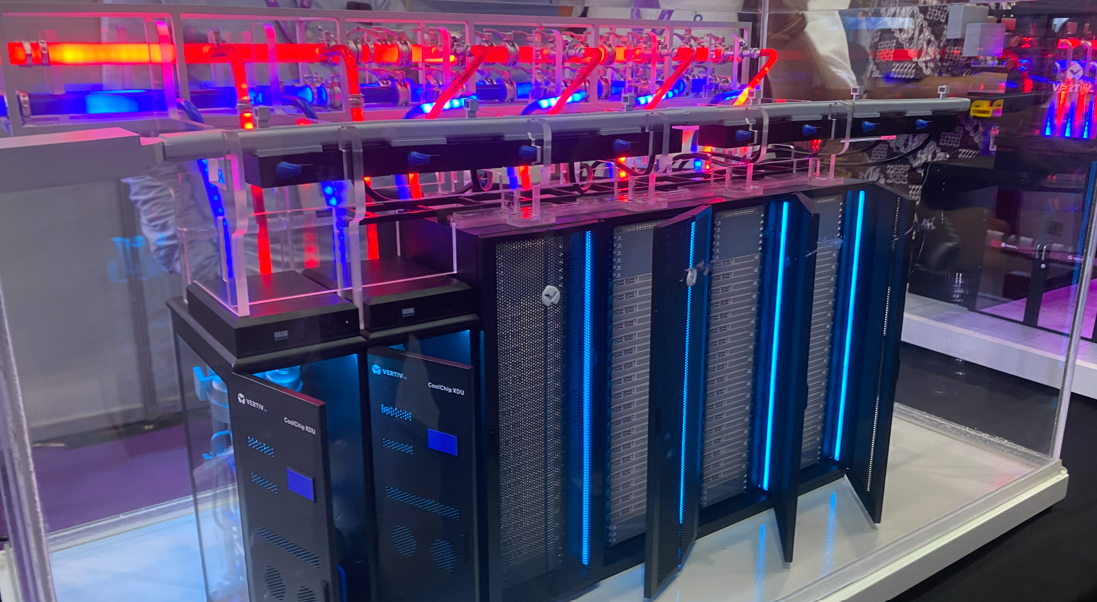
\includegraphics[width=0.85\textwidth]{images/kegiatan3.png}
    \caption{Dokumentasi kegiatan kerja praktik 3}
\end{figure}

\begin{figure}[H]
    \centering
    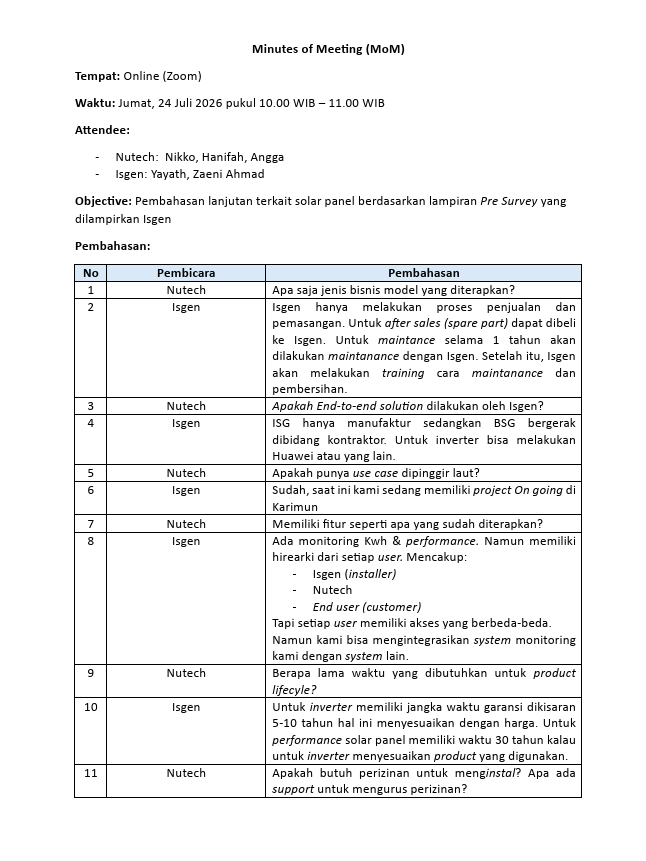
\includegraphics[width=0.85\textwidth]{images/MOM.png}
    \caption{Dokumentasi \textit{Minutes of Meeting} pembahasan solusi PJUTS}
\end{figure}

\begin{figure}[H]
    \centering
    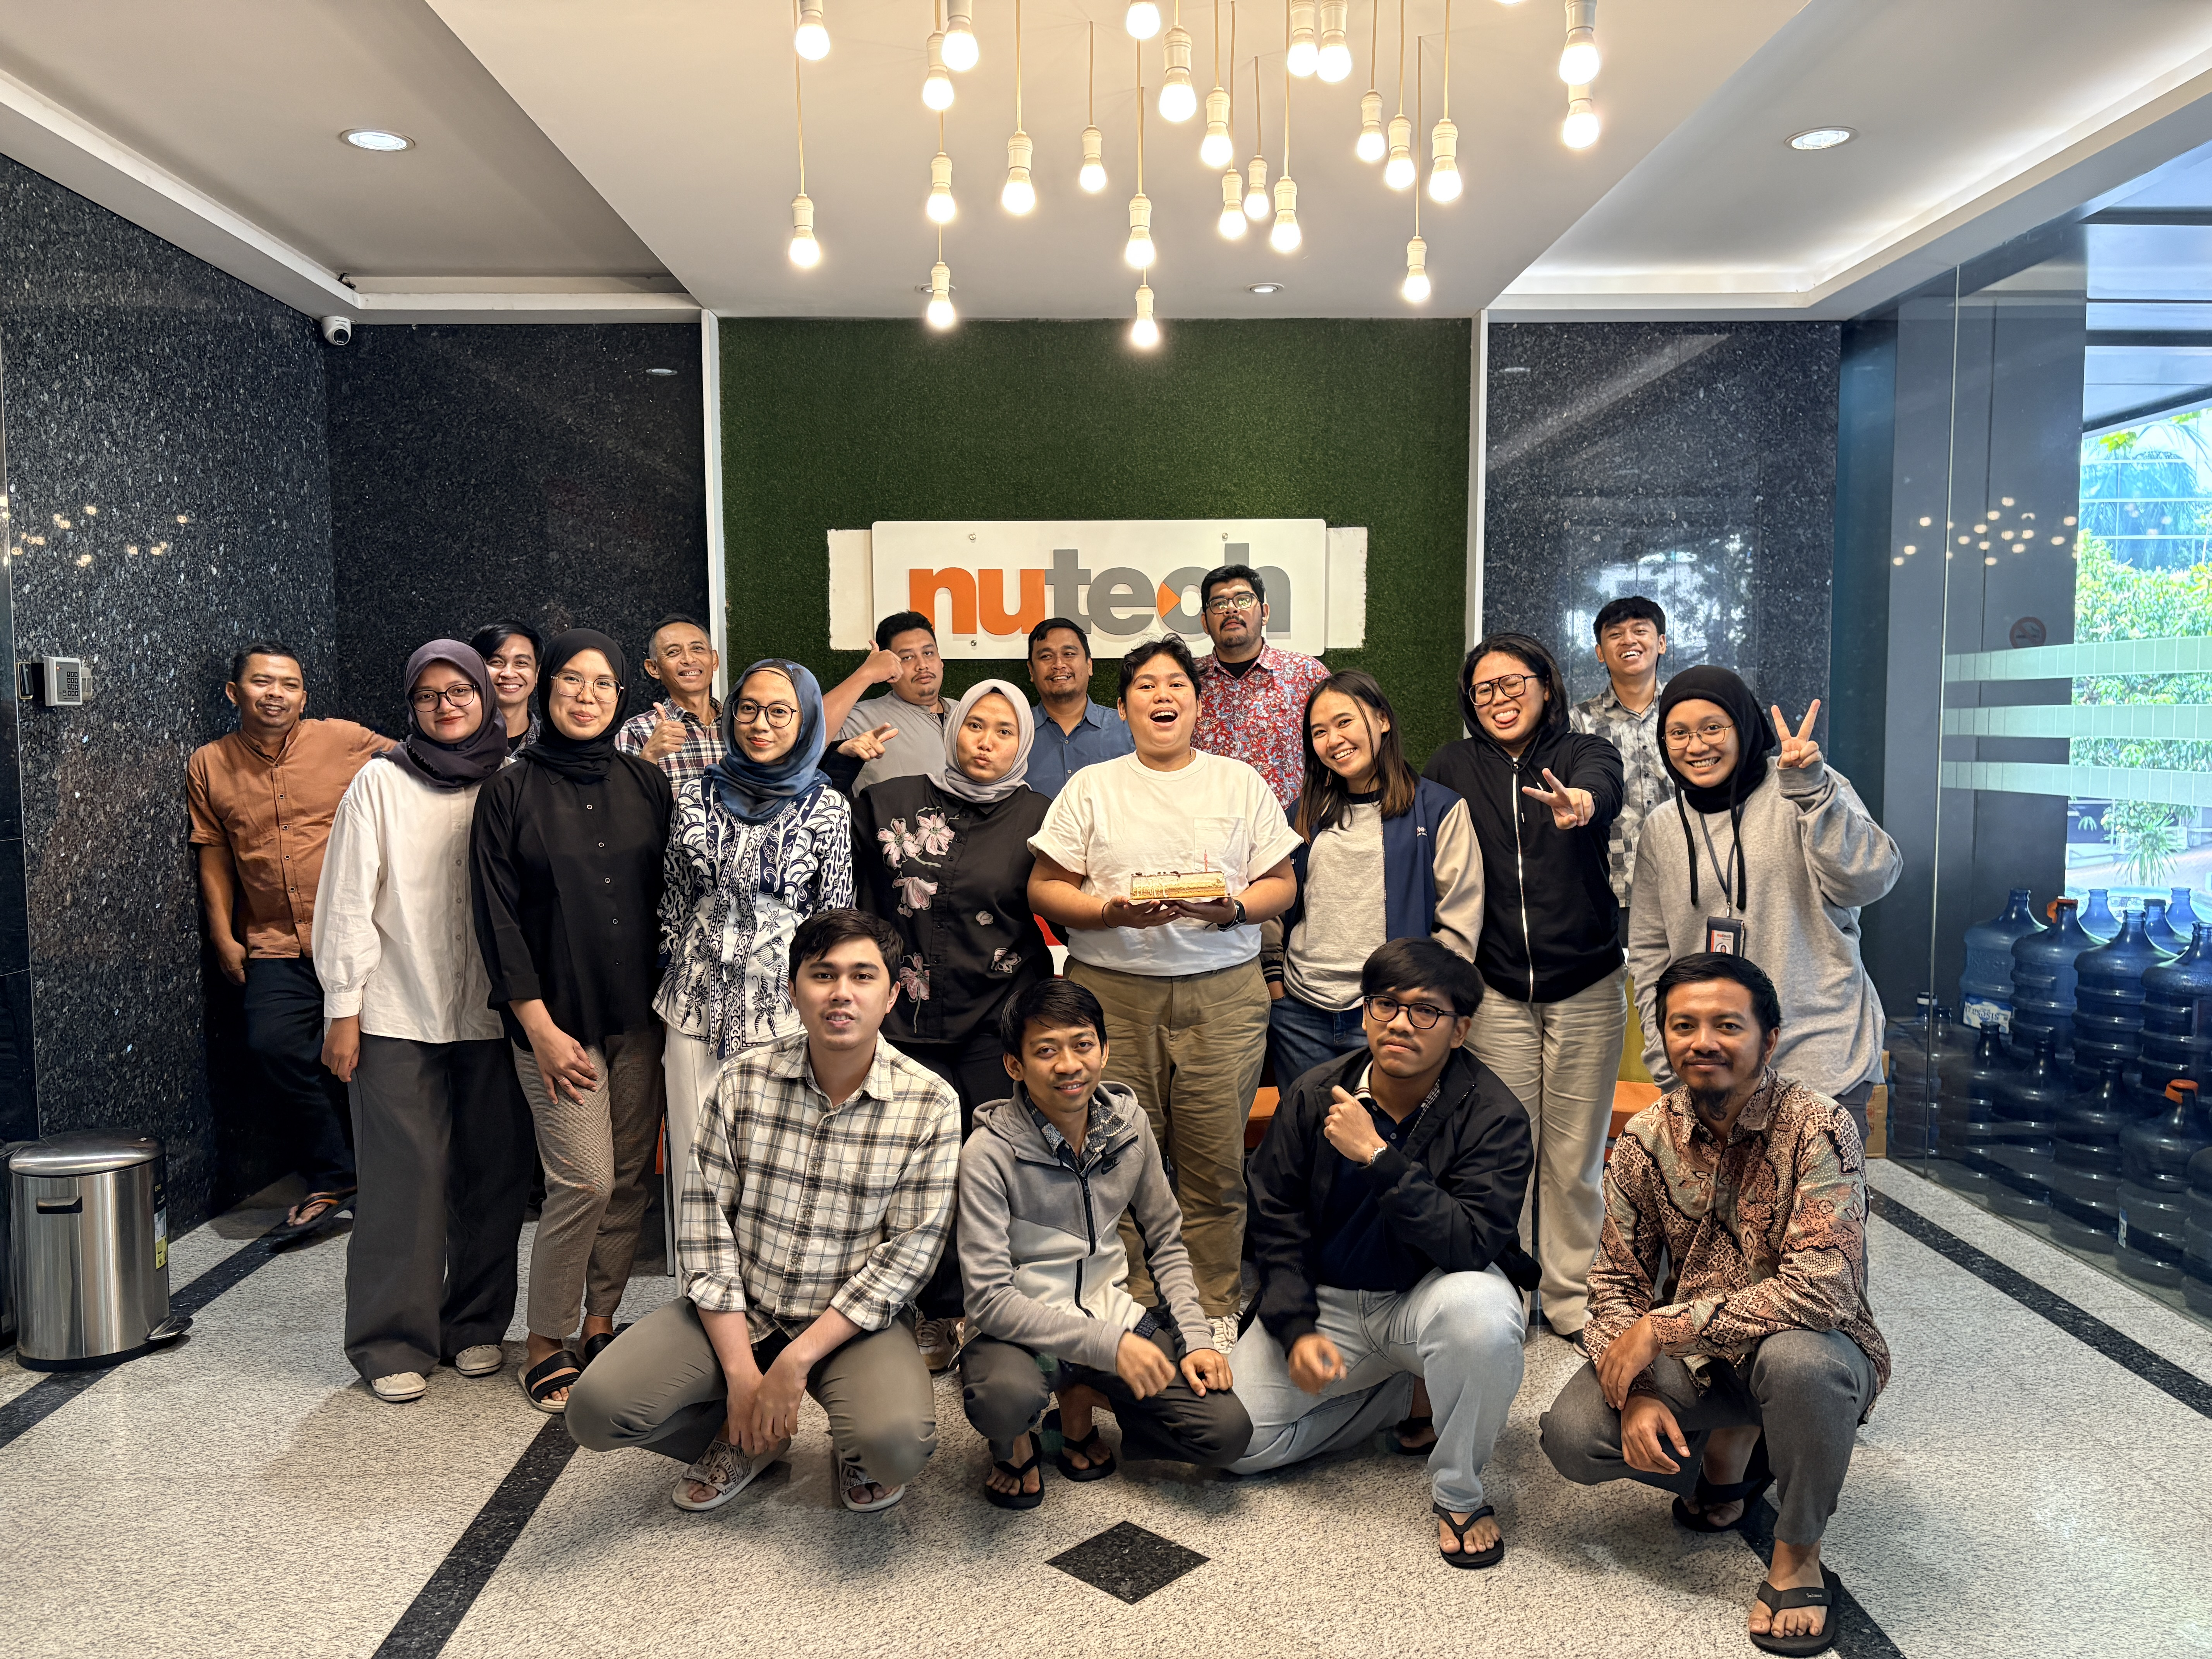
\includegraphics[width=0.85\textwidth]{images/perayaanultah.JPG}
    \caption{Perayaan ulang tahun rekan kerja}
\end{figure}

\begin{figure}[H]
    \centering
    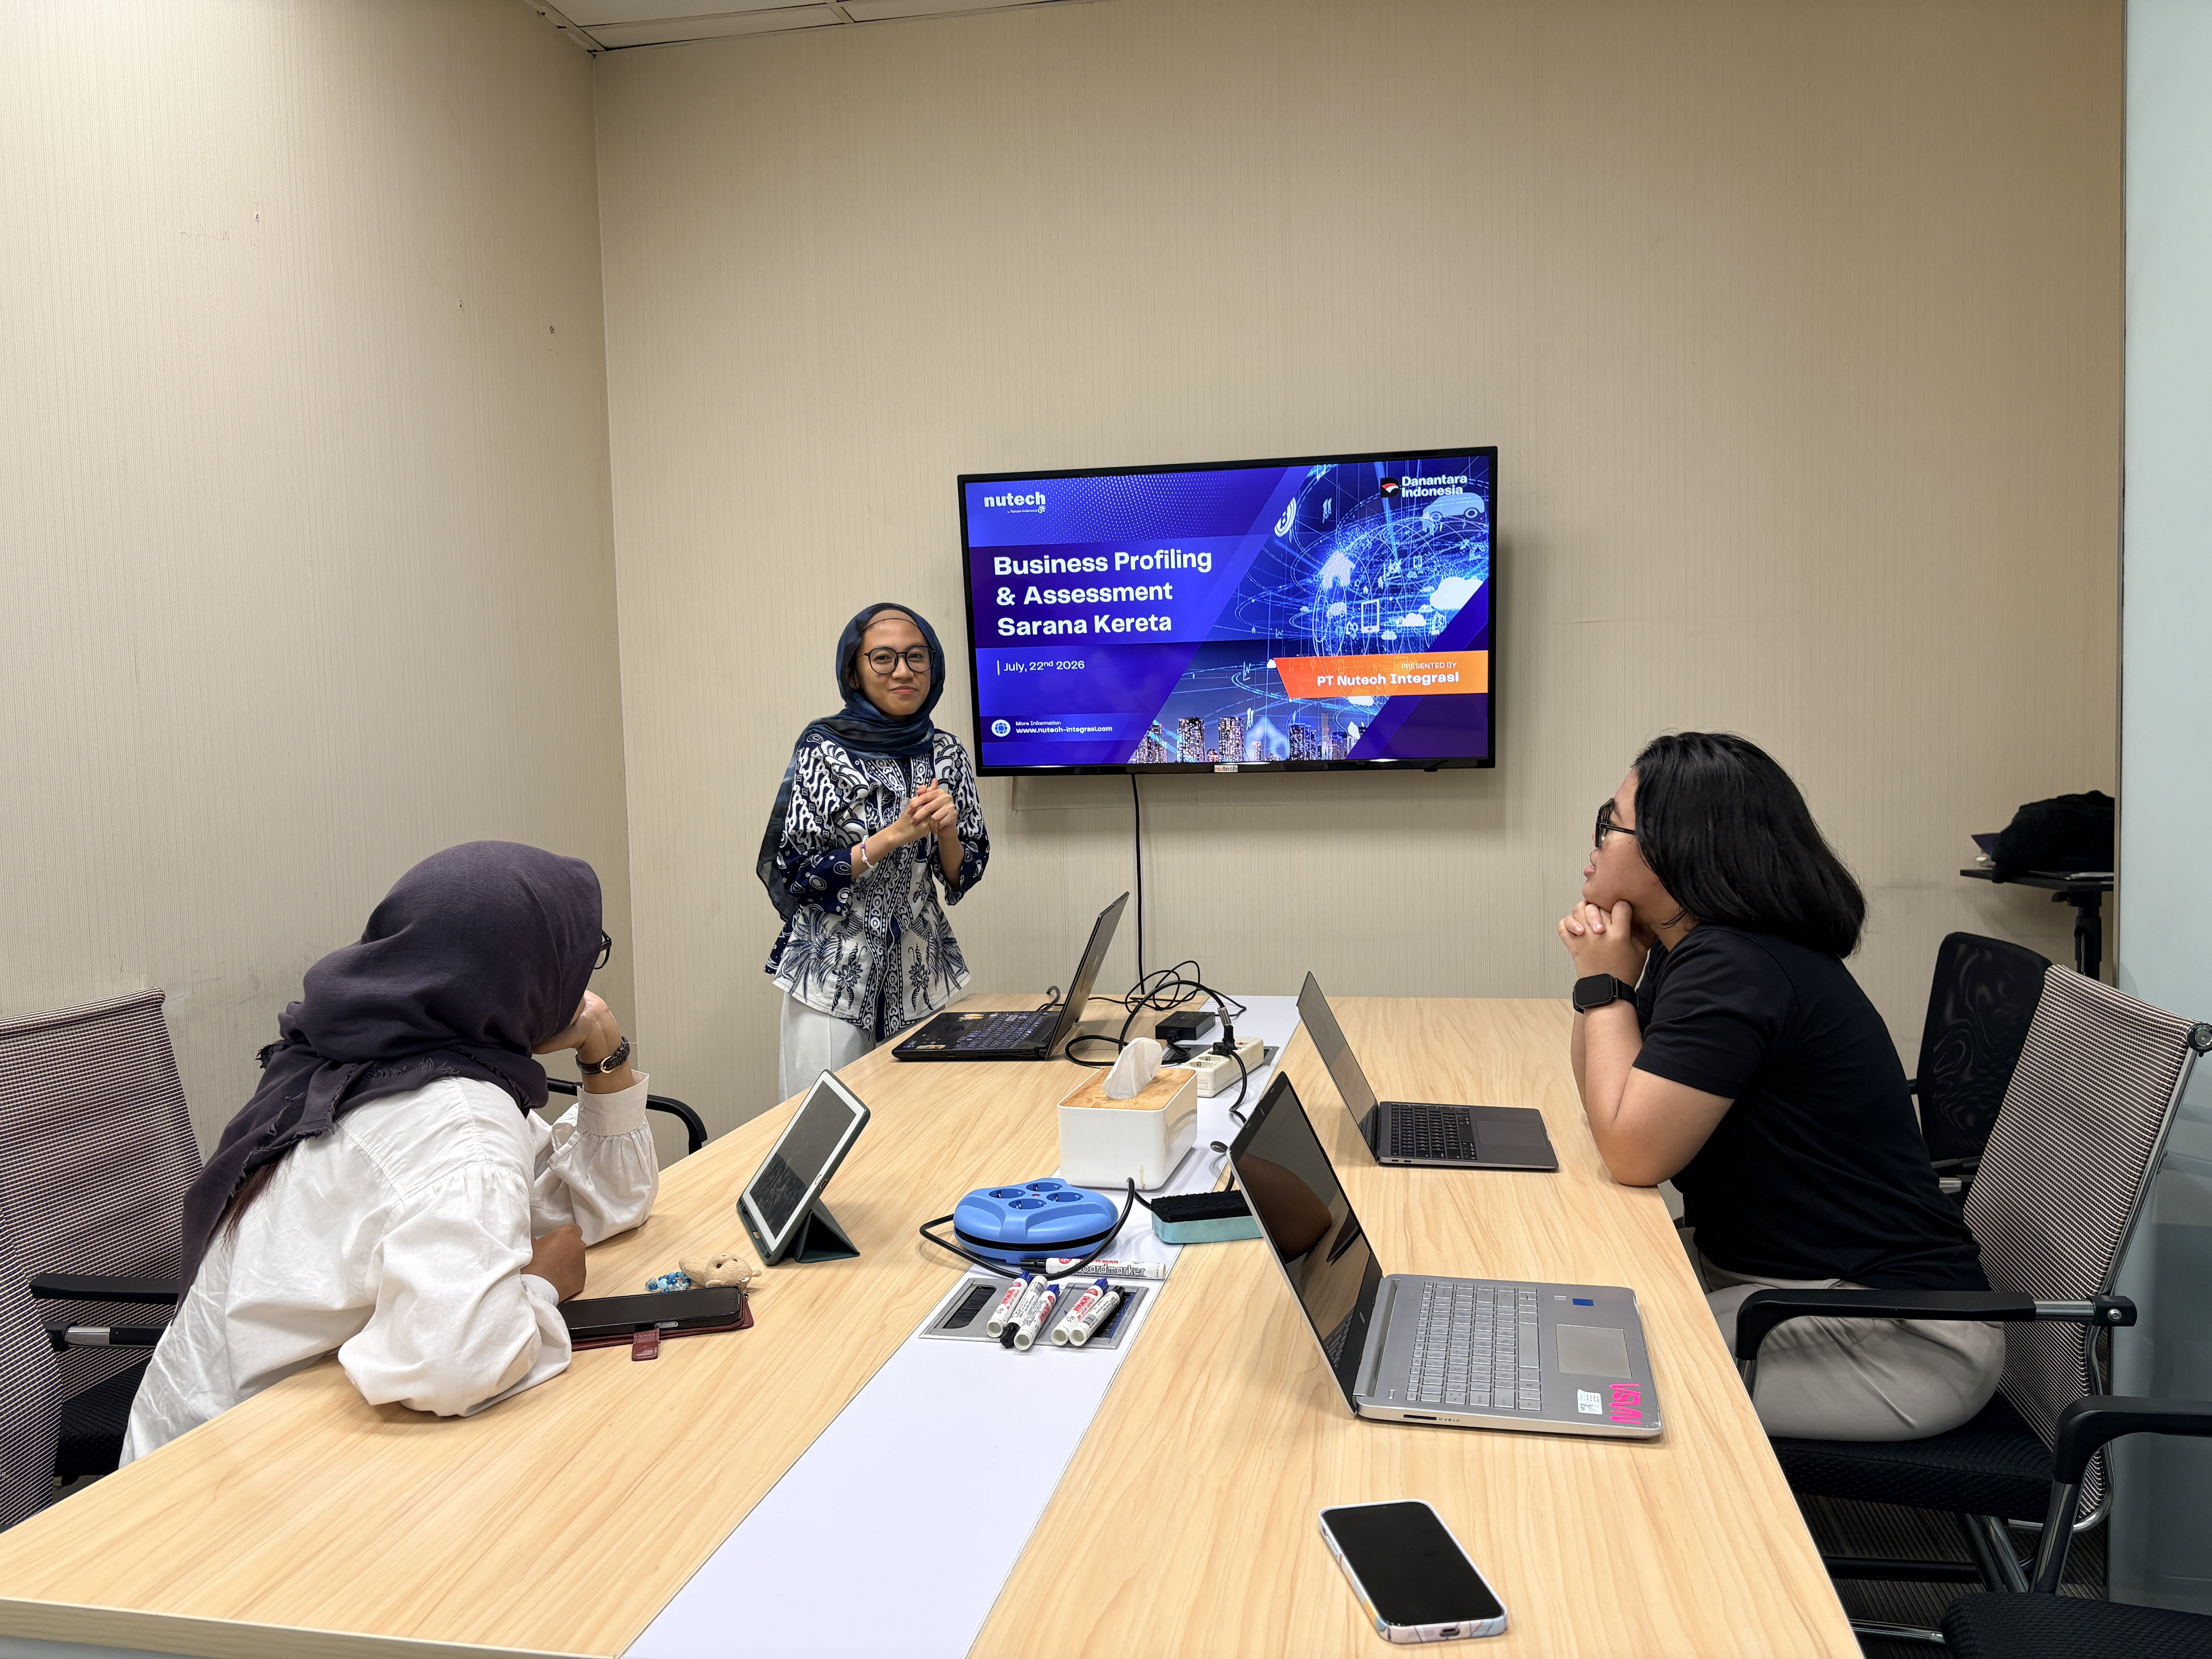
\includegraphics[width=0.85\textwidth]{images/presentasi1.JPG}
    \caption{Penyampaian presentasi hasil kerja praktik}
\end{figure}
